%Mimic Module

\subsubsection{Overview}
\label{Mimic}
\index{Mimic}\index{utilities, Mimic}

\begin{figure}[h]
\begin{center}
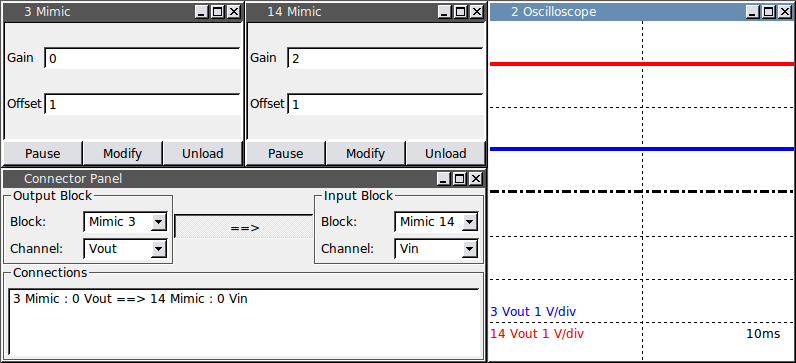
\includegraphics[width=4.5in]{mimic.png} 
\caption[Mimic]{Two Mimic modules are connected with their outputs displayed on the oscilloscope. Mimic-3, as shown in the blue oscilloscope trace, is outputting an offset of 1. As shown in the connector, Mimic-3's output (Vout) is connected to Mimic-14's (Vin). Mimic-14 applies the set gain and offset to Mimic-3's signal (1*2+1), resulting in an output of 4 shown in red. A tutorial is provided to replicate this figure.}
\end{center}
\label{mimic1}
\end{figure}
\seealso{Chapter \ref{mimic tutorial}\\Mimic Tutorial}

The Mimic module is the simplest signal generator available in RTXI. Mimic's main function is to apply a gain and/or offset to a signal it receives. By itself, Mimic can also be used output a continuous signal.

\subsubsection{Input Channels}
\begin{description}
\item [Vin]Gain and offset applied to this input to calculate output
\end{description}

\subsubsection{Output Channels}
\begin{description}
\item [Vout]Output calculated by multiplying input signal by gain and adding offset
\end{description}

\subsubsection{Parameters}
\begin{description}
\item [Gain]Factor by which input is multipled
\item [Offset]Factor added to the input. If no input is connected (i.e. input = 0), offset solely determines output
\end{description}

\subsubsection{Tutorial}
\label{mimic tutorial}\index{Mimic, tutorial}\index{tutorial, Mimic}
This tutorial is meant to be performed after the Signal Generator tutorial. The mimic module will be used to add a gain of 0.5 and offset of 1 to the biphasic square wave output by the signal generator.

\begin{enumerate}
\item Use the signal generator to output a biphasic square wave, where each phase is 1s long and has an amplitude of 4. Output this signal to the oscilloscope. These steps are covered in the Signal Generator tutorial. \seealso{Chapter \ref{siggen tutorial}\\Signal Generator Tutorial}
\item Open up a Mimic module through the menu: \textbf{Utilities}$\rightarrow$\textbf{Signals}$rightarrow$\textbf{Mimic}
\item Open the Connetor Panel through the menu: \textbf{System}$\rightarrow$\seealso{Chapter \ref{Connector}\\Connector}\textbf{Connector}
\item Connect the output of the Signal Generator module to the input of Mimic
  \begin{itemize}
  \item In the output block on the left side of the \textbf{Connector Panel}, select the Signal Generator module. The channel option should default to its only option, \textbf{Signal Waveform}
  \item In the input block on the right side of the \textbf{Connector Panel}, select the other Mimic module. The channel option should default to its only option, \textbf{Vin}
  \end{itemize}
\item Set up the oscilloscope to visualize the output of the Mimic module, in conjunction with the output of Signal Generator,  by right clicking on the oscilloscope and selecting \textbf{Properties}
  \begin{itemize}
  \item Make sure the \textbf{Channel} Tab is currently selected
  \item Select the Mimic module under the channel pulldown menu
  \item Select \textbf{Output} in the following pulldown menu, and make sure \textbf{Vout} is the selected output
  \item Activate the channel by hitting the toggle button \textbf{Active}
  \item Change the scale to \textbf{1 V/div} in the Scale pulldown menu
  \item Change the color to \textbf{Blue}
  \item Click the \textbf{Apply} button to save the changes
  \end{itemize}
\item Set the \textbf{Gain to 2} and the \textbf{Offset} to 1
\item Untoggle the \textbf{Pause} button
\item The output should now appear on the oscilloscope as in Figure \ref{mimic2}
\end{enumerate}

\begin{figure}[h]
\begin{center}
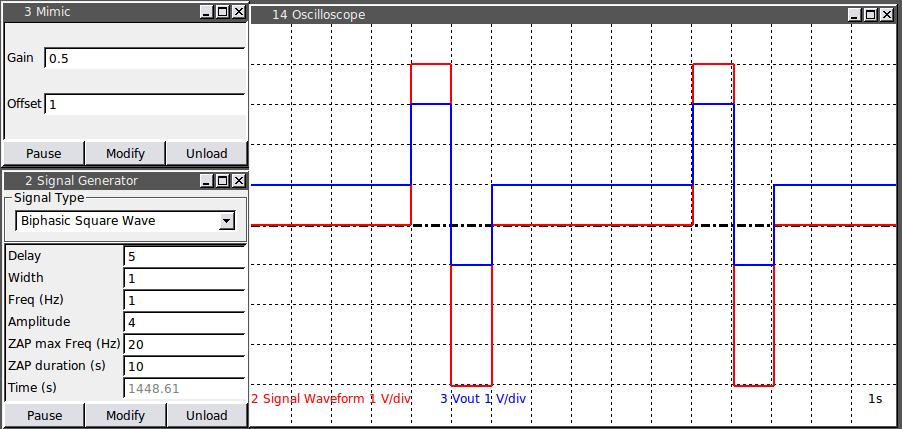
\includegraphics[width=4.5in]{mimic2.png} 
\caption[Mimic]{The Signal Generator module is outputting a biphasic square wave (red trace). This output is connected to the input of the Mimic module. The mimic module is applying a gain of 0.5 and an offset of 1 to the biphasic square, and outputs this modified signal (blue trace).}
\end{center}
\label{mimic2}
\end{figure}
\seealso{Chapter \ref{mimic tutorial}\\Mimic Tutorial}